\documentclass[1p]{elsarticle_modified}
%\bibliographystyle{elsarticle-num}

%\usepackage[colorlinks]{hyperref}
%\usepackage{abbrmath_seonhwa} %\Abb, \Ascr, \Acal ,\Abf, \Afrak
\usepackage{amsfonts}
\usepackage{amssymb}
\usepackage{amsmath}
\usepackage{amsthm}
\usepackage{scalefnt}
\usepackage{amsbsy}
\usepackage{kotex}
\usepackage{caption}
\usepackage{subfig}
\usepackage{color}
\usepackage{graphicx}
\usepackage{xcolor} %% white, black, red, green, blue, cyan, magenta, yellow
\usepackage{float}
\usepackage{setspace}
\usepackage{hyperref}

\usepackage{tikz}
\usetikzlibrary{arrows}

\usepackage{multirow}
\usepackage{array} % fixed length table
\usepackage{hhline}

%%%%%%%%%%%%%%%%%%%%%
\makeatletter
\renewcommand*\env@matrix[1][\arraystretch]{%
	\edef\arraystretch{#1}%
	\hskip -\arraycolsep
	\let\@ifnextchar\new@ifnextchar
	\array{*\c@MaxMatrixCols c}}
\makeatother %https://tex.stackexchange.com/questions/14071/how-can-i-increase-the-line-spacing-in-a-matrix
%%%%%%%%%%%%%%%

\usepackage[normalem]{ulem}

\newcommand{\msout}[1]{\ifmmode\text{\sout{\ensuremath{#1}}}\else\sout{#1}\fi}
%SOURCE: \msout is \stkout macro in https://tex.stackexchange.com/questions/20609/strikeout-in-math-mode

\newcommand{\cancel}[1]{
	\ifmmode
	{\color{red}\msout{#1}}
	\else
	{\color{red}\sout{#1}}
	\fi
}

\newcommand{\add}[1]{
	{\color{blue}\uwave{#1}}
}

\newcommand{\replace}[2]{
	\ifmmode
	{\color{red}\msout{#1}}{\color{blue}\uwave{#2}}
	\else
	{\color{red}\sout{#1}}{\color{blue}\uwave{#2}}
	\fi
}

\newcommand{\Sol}{\mathcal{S}} %segment
\newcommand{\D}{D} %diagram
\newcommand{\A}{\mathcal{A}} %arc


%%%%%%%%%%%%%%%%%%%%%%%%%%%%%5 test

\def\sl{\operatorname{\textup{SL}}(2,\Cbb)}
\def\psl{\operatorname{\textup{PSL}}(2,\Cbb)}
\def\quan{\mkern 1mu \triangleright \mkern 1mu}

\theoremstyle{definition}
\newtheorem{thm}{Theorem}[section]
\newtheorem{prop}[thm]{Proposition}
\newtheorem{lem}[thm]{Lemma}
\newtheorem{ques}[thm]{Question}
\newtheorem{cor}[thm]{Corollary}
\newtheorem{defn}[thm]{Definition}
\newtheorem{exam}[thm]{Example}
\newtheorem{rmk}[thm]{Remark}
\newtheorem{alg}[thm]{Algorithm}

\newcommand{\I}{\sqrt{-1}}
\begin{document}

%\begin{frontmatter}
%
%\title{Boundary parabolic representations of knots up to 8 crossings}
%
%%% Group authors per affiliation:
%\author{Yunhi Cho} 
%\address{Department of Mathematics, University of Seoul, Seoul, Korea}
%\ead{yhcho@uos.ac.kr}
%
%
%\author{Seonhwa Kim} %\fnref{s_kim}}
%\address{Center for Geometry and Physics, Institute for Basic Science, Pohang, 37673, Korea}
%\ead{ryeona17@ibs.re.kr}
%
%\author{Hyuk Kim}
%\address{Department of Mathematical Sciences, Seoul National University, Seoul 08826, Korea}
%\ead{hyukkim@snu.ac.kr}
%
%\author{Seokbeom Yoon}
%\address{Department of Mathematical Sciences, Seoul National University, Seoul, 08826,  Korea}
%\ead{sbyoon15@snu.ac.kr}
%
%\begin{abstract}
%We find all boundary parabolic representation of knots up to 8 crossings.
%
%\end{abstract}
%\begin{keyword}
%    \MSC[2010] 57M25 
%\end{keyword}
%
%\end{frontmatter}

%\linenumbers
%\tableofcontents
%
\newcommand\colored[1]{\textcolor{white}{\rule[-0.35ex]{0.8em}{1.4ex}}\kern-0.8em\color{red} #1}%
%\newcommand\colored[1]{\textcolor{white}{ #1}\kern-2.17ex	\textcolor{white}{ #1}\kern-1.81ex	\textcolor{white}{ #1}\kern-2.15ex\color{red}#1	}

{\Large $\underline{12a_{0197}~(K12a_{0197})}$}

\setlength{\tabcolsep}{10pt}
\renewcommand{\arraystretch}{1.6}
\vspace{1cm}\begin{tabular}{m{100pt}>{\centering\arraybackslash}m{274pt}}
\multirow{5}{120pt}{
	\centering
	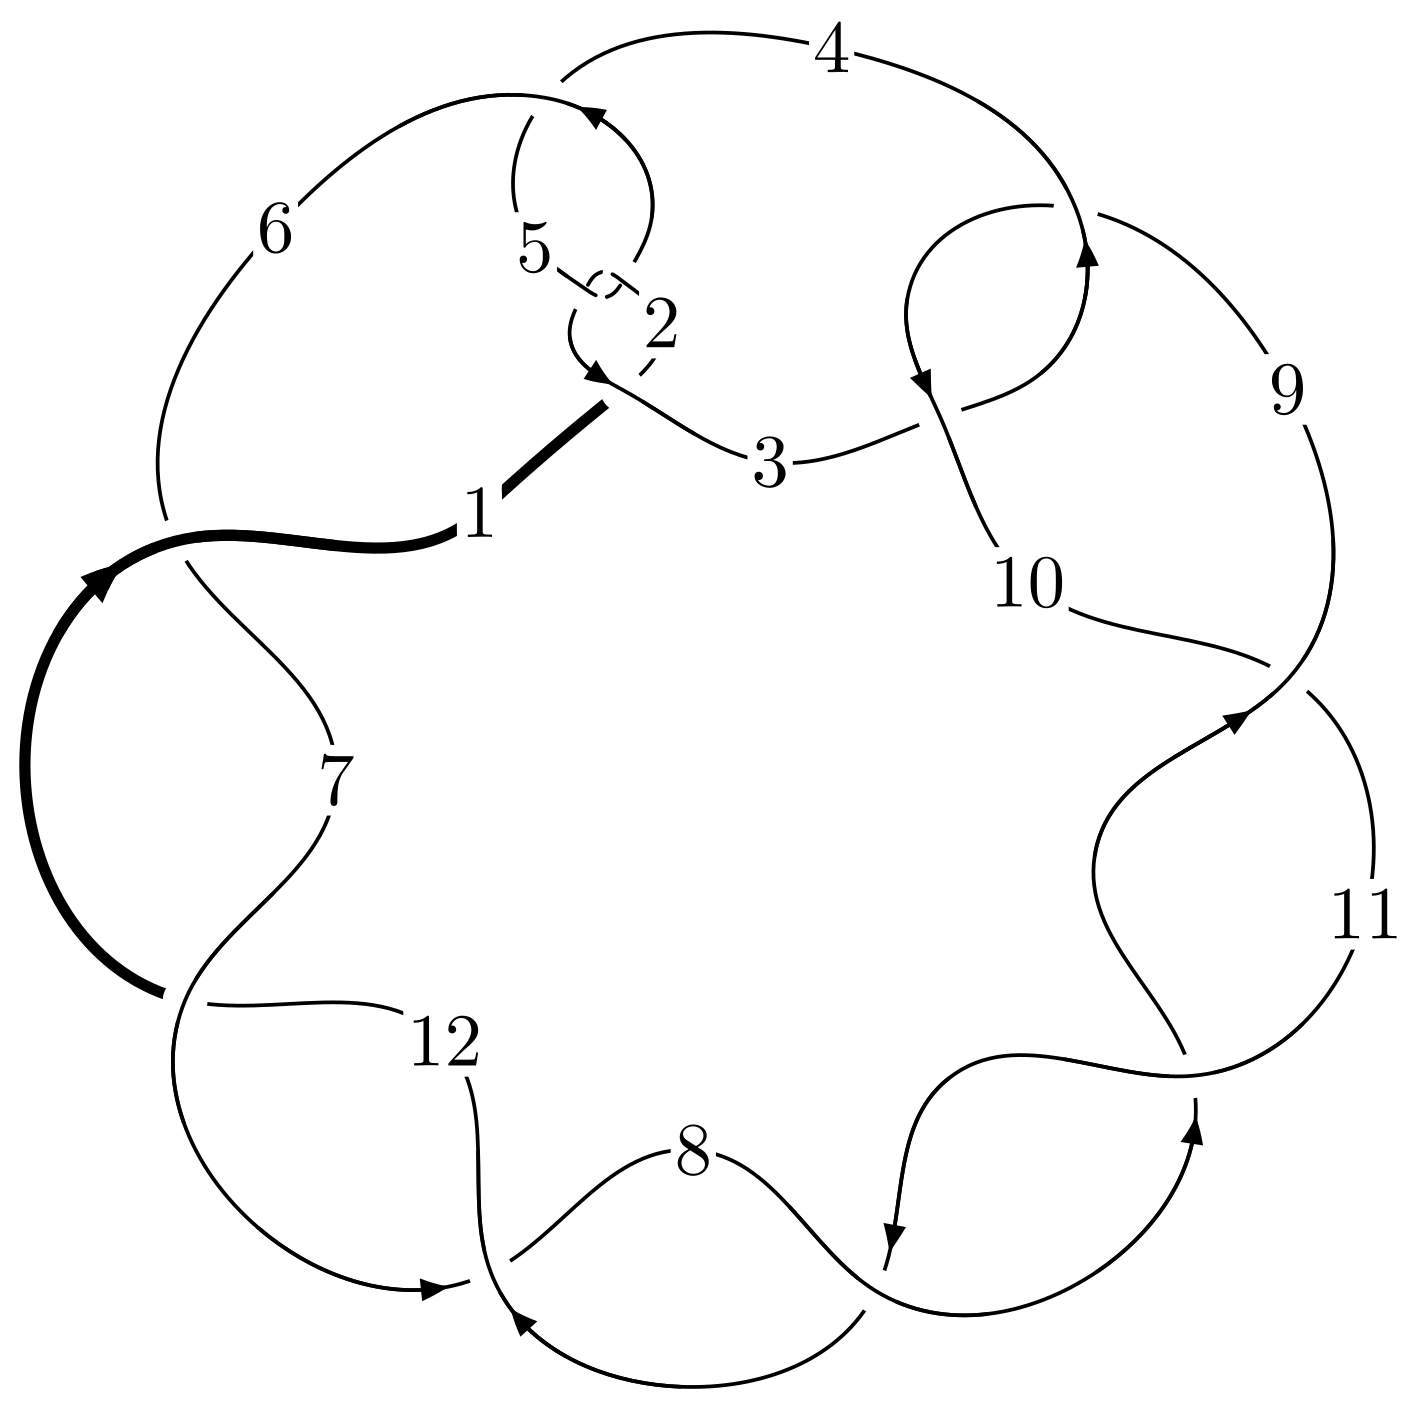
\includegraphics[width=112pt]{../../../GIT/diagram.site/Diagrams/png/998_12a_0197.png}\\
\ \ \ A knot diagram\footnotemark}&
\allowdisplaybreaks
\textbf{Linearized knot diagam} \\
\cline{2-2}
 &
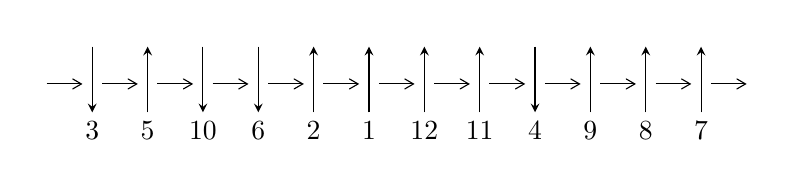
\begin{tikzpicture}[x=20pt, y=17pt]
	% nodes
	\node (C0) at (0, 0) {};
	\node (C1) at (1, 0) {};
	\node (C1U) at (1, +1) {};
	\node (C1D) at (1, -1) {3};

	\node (C2) at (2, 0) {};
	\node (C2U) at (2, +1) {};
	\node (C2D) at (2, -1) {5};

	\node (C3) at (3, 0) {};
	\node (C3U) at (3, +1) {};
	\node (C3D) at (3, -1) {10};

	\node (C4) at (4, 0) {};
	\node (C4U) at (4, +1) {};
	\node (C4D) at (4, -1) {6};

	\node (C5) at (5, 0) {};
	\node (C5U) at (5, +1) {};
	\node (C5D) at (5, -1) {2};

	\node (C6) at (6, 0) {};
	\node (C6U) at (6, +1) {};
	\node (C6D) at (6, -1) {1};

	\node (C7) at (7, 0) {};
	\node (C7U) at (7, +1) {};
	\node (C7D) at (7, -1) {12};

	\node (C8) at (8, 0) {};
	\node (C8U) at (8, +1) {};
	\node (C8D) at (8, -1) {11};

	\node (C9) at (9, 0) {};
	\node (C9U) at (9, +1) {};
	\node (C9D) at (9, -1) {4};

	\node (C10) at (10, 0) {};
	\node (C10U) at (10, +1) {};
	\node (C10D) at (10, -1) {9};

	\node (C11) at (11, 0) {};
	\node (C11U) at (11, +1) {};
	\node (C11D) at (11, -1) {8};

	\node (C12) at (12, 0) {};
	\node (C12U) at (12, +1) {};
	\node (C12D) at (12, -1) {7};
	\node (C13) at (13, 0) {};

	% arrows
	\draw[->,>={angle 60}]
	(C0) edge (C1) (C1) edge (C2) (C2) edge (C3) (C3) edge (C4) (C4) edge (C5) (C5) edge (C6) (C6) edge (C7) (C7) edge (C8) (C8) edge (C9) (C9) edge (C10) (C10) edge (C11) (C11) edge (C12) (C12) edge (C13) ;	\draw[->,>=stealth]
	(C1U) edge (C1D) (C2D) edge (C2U) (C3U) edge (C3D) (C4U) edge (C4D) (C5D) edge (C5U) (C6D) edge (C6U) (C7D) edge (C7U) (C8D) edge (C8U) (C9U) edge (C9D) (C10D) edge (C10U) (C11D) edge (C11U) (C12D) edge (C12U) ;
	\end{tikzpicture} \\
\hhline{~~} \\& 
\textbf{Solving Sequence} \\ \cline{2-2} 
 &
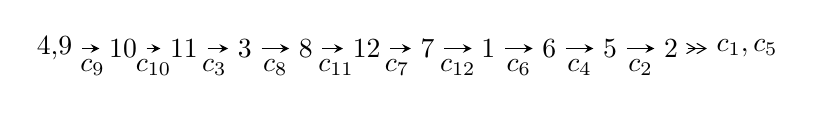
\begin{tikzpicture}[x=22pt, y=7pt]
	% node
	\node (A0) at (-1/8, 0) {4,9};
	\node (A1) at (1, 0) {10};
	\node (A2) at (2, 0) {11};
	\node (A3) at (3, 0) {3};
	\node (A4) at (4, 0) {8};
	\node (A5) at (5, 0) {12};
	\node (A6) at (6, 0) {7};
	\node (A7) at (7, 0) {1};
	\node (A8) at (8, 0) {6};
	\node (A9) at (9, 0) {5};
	\node (A10) at (10, 0) {2};
	\node (C1) at (1/2, -1) {$c_{9}$};
	\node (C2) at (3/2, -1) {$c_{10}$};
	\node (C3) at (5/2, -1) {$c_{3}$};
	\node (C4) at (7/2, -1) {$c_{8}$};
	\node (C5) at (9/2, -1) {$c_{11}$};
	\node (C6) at (11/2, -1) {$c_{7}$};
	\node (C7) at (13/2, -1) {$c_{12}$};
	\node (C8) at (15/2, -1) {$c_{6}$};
	\node (C9) at (17/2, -1) {$c_{4}$};
	\node (C10) at (19/2, -1) {$c_{2}$};
	\node (A11) at (45/4, 0) {$c_{1},c_{5}$};

	% edge
	\draw[->,>=stealth]	
	(A0) edge (A1) (A1) edge (A2) (A2) edge (A3) (A3) edge (A4) (A4) edge (A5) (A5) edge (A6) (A6) edge (A7) (A7) edge (A8) (A8) edge (A9) (A9) edge (A10) ;
	\draw[->>,>={angle 60}]	
	(A10) edge (A11);
\end{tikzpicture} \\ 

\end{tabular} \\

\footnotetext{
The image of knot diagram is generated by the software ``\textbf{Draw programme}" developed by Andrew Bartholomew(\url{http://www.layer8.co.uk/maths/draw/index.htm\#Running-draw}), where we modified some parts for our purpose(\url{https://github.com/CATsTAILs/LinksPainter}).
}\phantom \\ \newline 
\centering \textbf{Ideals for irreducible components\footnotemark of $X_{\text{par}}$} 
 
\begin{align*}
I^u_{1}&=\langle 
u^{34}+u^{33}+\cdots- u+1\rangle \\
\\
\end{align*}
\raggedright * 1 irreducible components of $\dim_{\mathbb{C}}=0$, with total 34 representations.\\
\footnotetext{All coefficients of polynomials are rational numbers. But the coefficients are sometimes approximated in decimal forms when there is not enough margin.}
\newpage
\renewcommand{\arraystretch}{1}
\centering \section*{I. $I^u_{1}= \langle u^{34}+u^{33}+\cdots- u+1 \rangle$}
\flushleft \textbf{(i) Arc colorings}\\
\begin{tabular}{m{7pt} m{180pt} m{7pt} m{180pt} }
\flushright $a_{4}=$&$\begin{pmatrix}0\\u\end{pmatrix}$ \\
\flushright $a_{9}=$&$\begin{pmatrix}1\\0\end{pmatrix}$ \\
\flushright $a_{10}=$&$\begin{pmatrix}1\\u^2\end{pmatrix}$ \\
\flushright $a_{11}=$&$\begin{pmatrix}u^2+1\\u^2\end{pmatrix}$ \\
\flushright $a_{3}=$&$\begin{pmatrix}u\\u^3+u\end{pmatrix}$ \\
\flushright $a_{8}=$&$\begin{pmatrix}u^4+u^2+1\\u^4\end{pmatrix}$ \\
\flushright $a_{12}=$&$\begin{pmatrix}u^6+u^4+2 u^2+1\\u^6+u^2\end{pmatrix}$ \\
\flushright $a_{7}=$&$\begin{pmatrix}u^8+u^6+3 u^4+2 u^2+1\\u^8+2 u^4\end{pmatrix}$ \\
\flushright $a_{1}=$&$\begin{pmatrix}u^{10}+u^8+4 u^6+3 u^4+3 u^2+1\\u^{10}+3 u^6+u^2\end{pmatrix}$ \\
\flushright $a_{6}=$&$\begin{pmatrix}u^{12}+u^{10}+5 u^8+4 u^6+6 u^4+3 u^2+1\\u^{12}+4 u^8+3 u^4\end{pmatrix}$ \\
\flushright $a_{5}=$&$\begin{pmatrix}- u^{25}-2 u^{23}+\cdots-6 u^3- u\\- u^{25}- u^{23}+\cdots-3 u^5+u\end{pmatrix}$ \\
\flushright $a_{2}=$&$\begin{pmatrix}u^{14}+u^{12}+6 u^{10}+5 u^8+10 u^6+6 u^4+4 u^2+1\\u^{16}+2 u^{14}+6 u^{12}+10 u^{10}+10 u^8+12 u^6+4 u^4+2 u^2\end{pmatrix}$\\&\end{tabular}
\flushleft \textbf{(ii) Obstruction class $= -1$}\\~\\
\flushleft \textbf{(iii) Cusp Shapes $= 4 u^{32}+4 u^{31}+12 u^{30}+8 u^{29}+64 u^{28}+52 u^{27}+144 u^{26}+88 u^{25}+396 u^{24}+268 u^{23}+676 u^{22}+376 u^{21}+1216 u^{20}+696 u^{19}+1564 u^{18}+784 u^{17}+1956 u^{16}+948 u^{15}+1836 u^{14}+812 u^{13}+1576 u^{12}+620 u^{11}+992 u^{10}+360 u^9+528 u^8+132 u^7+176 u^6+40 u^5+40 u^4-8 u^3+12 u^2+8 u+2$}\\~\\
\newpage\renewcommand{\arraystretch}{1}
\flushleft \textbf{(iv) u-Polynomials at the component}\newline \\
\begin{tabular}{m{50pt}|m{274pt}}
Crossings & \hspace{64pt}u-Polynomials at each crossing \\
\hline $$\begin{aligned}c_{1},c_{4}\end{aligned}$$&$\begin{aligned}
&u^{34}+13 u^{33}+\cdots+5 u+1
\end{aligned}$\\
\hline $$\begin{aligned}c_{2},c_{5}\end{aligned}$$&$\begin{aligned}
&u^{34}+u^{33}+\cdots-3 u+1
\end{aligned}$\\
\hline $$\begin{aligned}c_{3},c_{9}\end{aligned}$$&$\begin{aligned}
&u^{34}- u^{33}+\cdots+u+1
\end{aligned}$\\
\hline $$\begin{aligned}c_{6},c_{7},c_{8}\\c_{10},c_{11},c_{12}\end{aligned}$$&$\begin{aligned}
&u^{34}-5 u^{33}+\cdots-5 u+1
\end{aligned}$\\
\hline
\end{tabular}\\~\\
\newpage\renewcommand{\arraystretch}{1}
\flushleft \textbf{(v) Riley Polynomials at the component}\newline \\
\begin{tabular}{m{50pt}|m{274pt}}
Crossings & \hspace{64pt}Riley Polynomials at each crossing \\
\hline $$\begin{aligned}c_{1},c_{4}\end{aligned}$$&$\begin{aligned}
&y^{34}+17 y^{33}+\cdots+97 y+1
\end{aligned}$\\
\hline $$\begin{aligned}c_{2},c_{5}\end{aligned}$$&$\begin{aligned}
&y^{34}+13 y^{33}+\cdots+5 y+1
\end{aligned}$\\
\hline $$\begin{aligned}c_{3},c_{9}\end{aligned}$$&$\begin{aligned}
&y^{34}+5 y^{33}+\cdots+5 y+1
\end{aligned}$\\
\hline $$\begin{aligned}c_{6},c_{7},c_{8}\\c_{10},c_{11},c_{12}\end{aligned}$$&$\begin{aligned}
&y^{34}+49 y^{33}+\cdots+25 y+1
\end{aligned}$\\
\hline
\end{tabular}\\~\\
\newpage\flushleft \textbf{(vi) Complex Volumes and Cusp Shapes}
$$\begin{array}{c|c|c}  
\text{Solutions to }I^u_{1}& \I (\text{vol} + \sqrt{-1}CS) & \text{Cusp shape}\\
 \hline 
\begin{aligned}
u &= -0.407066 + 0.834658 I\end{aligned}
 & \phantom{-}1.03103 + 6.41382 I & \phantom{-}3.82648 - 9.99401 I \\ \hline\begin{aligned}
u &= -0.407066 - 0.834658 I\end{aligned}
 & \phantom{-}1.03103 - 6.41382 I & \phantom{-}3.82648 + 9.99401 I \\ \hline\begin{aligned}
u &= -0.760333 + 0.772672 I\end{aligned}
 & -4.35750 + 1.50466 I & \phantom{-}0.22640 - 2.73870 I \\ \hline\begin{aligned}
u &= -0.760333 - 0.772672 I\end{aligned}
 & -4.35750 - 1.50466 I & \phantom{-}0.22640 + 2.73870 I \\ \hline\begin{aligned}
u &= \phantom{-}0.802505 + 0.764339 I\end{aligned}
 & -5.87304 + 3.61528 I & -2.19692 - 2.52505 I \\ \hline\begin{aligned}
u &= \phantom{-}0.802505 - 0.764339 I\end{aligned}
 & -5.87304 - 3.61528 I & -2.19692 + 2.52505 I \\ \hline\begin{aligned}
u &= \phantom{-}0.348058 + 0.805715 I\end{aligned}
 & \phantom{-}1.73732 - 1.33000 I & \phantom{-}6.22240 + 4.49160 I \\ \hline\begin{aligned}
u &= \phantom{-}0.348058 - 0.805715 I\end{aligned}
 & \phantom{-}1.73732 + 1.33000 I & \phantom{-}6.22240 - 4.49160 I \\ \hline\begin{aligned}
u &= -0.718616 + 0.868268 I\end{aligned}
 & -4.04046 + 3.96737 I & \phantom{-}1.07736 - 3.54418 I \\ \hline\begin{aligned}
u &= -0.718616 - 0.868268 I\end{aligned}
 & -4.04046 - 3.96737 I & \phantom{-}1.07736 + 3.54418 I \\ \hline\begin{aligned}
u &= -0.532857 + 0.661540 I\end{aligned}
 & -2.87697 + 1.94550 I & -4.75114 - 5.05594 I \\ \hline\begin{aligned}
u &= -0.532857 - 0.661540 I\end{aligned}
 & -2.87697 - 1.94550 I & -4.75114 + 5.05594 I \\ \hline\begin{aligned}
u &= \phantom{-}0.786286 + 0.843735 I\end{aligned}
 & -9.58813 - 2.89200 I & -5.67849 + 3.04986 I \\ \hline\begin{aligned}
u &= \phantom{-}0.786286 - 0.843735 I\end{aligned}
 & -9.58813 + 2.89200 I & -5.67849 - 3.04986 I \\ \hline\begin{aligned}
u &= \phantom{-}0.733686 + 0.898055 I\end{aligned}
 & -5.42158 - 9.27208 I & -0.93638 + 8.29994 I \\ \hline\begin{aligned}
u &= \phantom{-}0.733686 - 0.898055 I\end{aligned}
 & -5.42158 + 9.27208 I & -0.93638 - 8.29994 I \\ \hline\begin{aligned}
u &= \phantom{-}0.034944 + 0.814547 I\end{aligned}
 & \phantom{-}3.24779 - 2.53240 I & \phantom{-}10.48060 + 3.91593 I \\ \hline\begin{aligned}
u &= \phantom{-}0.034944 - 0.814547 I\end{aligned}
 & \phantom{-}3.24779 + 2.53240 I & \phantom{-}10.48060 - 3.91593 I \\ \hline\begin{aligned}
u &= -0.560898 + 0.384252 I\end{aligned}
 & -0.40745 - 2.89261 I & -2.01184 + 2.94776 I \\ \hline\begin{aligned}
u &= -0.560898 - 0.384252 I\end{aligned}
 & -0.40745 + 2.89261 I & -2.01184 - 2.94776 I \\ \hline\begin{aligned}
u &= \phantom{-}0.943944 + 0.946247 I\end{aligned}
 & -15.2642 - 1.6043 I & \phantom{-}0.05765 + 2.13250 I \\ \hline\begin{aligned}
u &= \phantom{-}0.943944 - 0.946247 I\end{aligned}
 & -15.2642 + 1.6043 I & \phantom{-}0.05765 - 2.13250 I \\ \hline\begin{aligned}
u &= -0.951432 + 0.943931 I\end{aligned}
 & -17.0241 - 3.9437 I & -2.23878 + 2.32500 I \\ \hline\begin{aligned}
u &= -0.951432 - 0.943931 I\end{aligned}
 & -17.0241 + 3.9437 I & -2.23878 - 2.32500 I \\ \hline\begin{aligned}
u &= \phantom{-}0.933375 + 0.963881 I\end{aligned}
 & -15.2051 - 5.2894 I & \phantom{-}0.15464 + 2.30279 I \\ \hline\begin{aligned}
u &= \phantom{-}0.933375 - 0.963881 I\end{aligned}
 & -15.2051 + 5.2894 I & \phantom{-}0.15464 - 2.30279 I \\ \hline\begin{aligned}
u &= -0.934696 + 0.971112 I\end{aligned}
 & -16.9325 + 10.8664 I & -2.05453 - 6.71778 I \\ \hline\begin{aligned}
u &= -0.934696 - 0.971112 I\end{aligned}
 & -16.9325 - 10.8664 I & -2.05453 + 6.71778 I \\ \hline\begin{aligned}
u &= -0.946814 + 0.960125 I\end{aligned}
 & \phantom{-}18.2073 + 3.4743 I & -5.57472 - 2.21410 I \\ \hline\begin{aligned}
u &= -0.946814 - 0.960125 I\end{aligned}
 & \phantom{-}18.2073 - 3.4743 I & -5.57472 + 2.21410 I\\
 \hline 
 \end{array}$$\newpage$$\begin{array}{c|c|c}  
\text{Solutions to }I^u_{1}& \I (\text{vol} + \sqrt{-1}CS) & \text{Cusp shape}\\
 \hline 
\begin{aligned}
u &= \phantom{-}0.258906 + 0.569344 I\end{aligned}
 & \phantom{-}0.245296 - 0.924586 I & \phantom{-}4.90419 + 7.15131 I \\ \hline\begin{aligned}
u &= \phantom{-}0.258906 - 0.569344 I\end{aligned}
 & \phantom{-}0.245296 + 0.924586 I & \phantom{-}4.90419 - 7.15131 I \\ \hline\begin{aligned}
u &= \phantom{-}0.471008 + 0.235567 I\end{aligned}
 & \phantom{-}0.14514 - 1.57341 I & -1.50693 + 3.59818 I \\ \hline\begin{aligned}
u &= \phantom{-}0.471008 - 0.235567 I\end{aligned}
 & \phantom{-}0.14514 + 1.57341 I & -1.50693 - 3.59818 I\\
 \hline 
 \end{array}$$\newpage
\newpage\renewcommand{\arraystretch}{1}
\centering \section*{ II. u-Polynomials}
\begin{tabular}{m{50pt}|m{274pt}}
Crossings & \hspace{64pt}u-Polynomials at each crossing \\
\hline $$\begin{aligned}c_{1},c_{4}\end{aligned}$$&$\begin{aligned}
&u^{34}+13 u^{33}+\cdots+5 u+1
\end{aligned}$\\
\hline $$\begin{aligned}c_{2},c_{5}\end{aligned}$$&$\begin{aligned}
&u^{34}+u^{33}+\cdots-3 u+1
\end{aligned}$\\
\hline $$\begin{aligned}c_{3},c_{9}\end{aligned}$$&$\begin{aligned}
&u^{34}- u^{33}+\cdots+u+1
\end{aligned}$\\
\hline $$\begin{aligned}c_{6},c_{7},c_{8}\\c_{10},c_{11},c_{12}\end{aligned}$$&$\begin{aligned}
&u^{34}-5 u^{33}+\cdots-5 u+1
\end{aligned}$\\
\hline
\end{tabular}\newpage\renewcommand{\arraystretch}{1}
\centering \section*{ III. Riley Polynomials}
\begin{tabular}{m{50pt}|m{274pt}}
Crossings & \hspace{64pt}Riley Polynomials at each crossing \\
\hline $$\begin{aligned}c_{1},c_{4}\end{aligned}$$&$\begin{aligned}
&y^{34}+17 y^{33}+\cdots+97 y+1
\end{aligned}$\\
\hline $$\begin{aligned}c_{2},c_{5}\end{aligned}$$&$\begin{aligned}
&y^{34}+13 y^{33}+\cdots+5 y+1
\end{aligned}$\\
\hline $$\begin{aligned}c_{3},c_{9}\end{aligned}$$&$\begin{aligned}
&y^{34}+5 y^{33}+\cdots+5 y+1
\end{aligned}$\\
\hline $$\begin{aligned}c_{6},c_{7},c_{8}\\c_{10},c_{11},c_{12}\end{aligned}$$&$\begin{aligned}
&y^{34}+49 y^{33}+\cdots+25 y+1
\end{aligned}$\\
\hline
\end{tabular}
\vskip 2pc
\end{document}